\chapter{Théorie semi-classique des laser}
\section{Équations de Maxwell-Bloch du laser}
Classique : le champ EM est décrit par les équations de Maxwell
\begin{equation}
\Delta E - \frac{1}{{{{\rm{c}}^2}}}\frac{{{\partial ^2}}}{{\partial {t^2}}}E = {\rm{ }}{\mu _0}\frac{{{\partial ^2}}}{{\partial {t^2}}}P
\end{equation}

\begin{center}
	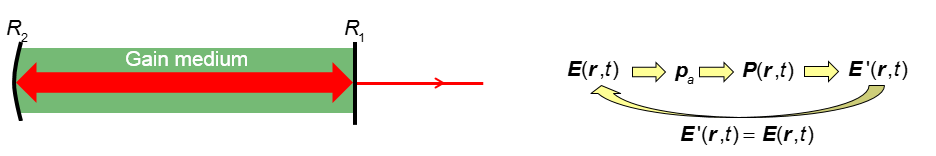
\includegraphics[scale=0.65]{ch3/image1.png}
	\captionof{figure}{ }
\end{center}
Il existe un couplage entre la radiation et le milieu : le champ électrique introduit une 
polarisation atomique qui induit un champ de polarisation macroscopique qui elle même 
donne lieu au champ électrique total, la boucle recommence alors.

\subsection{Équations du champ électromagnétique dans la cavité}
\subsubsection{Mode longitudinal de la cavité}
	\begin{wrapfigure}[7]{r}{8cm}
	\vspace{-5mm}
	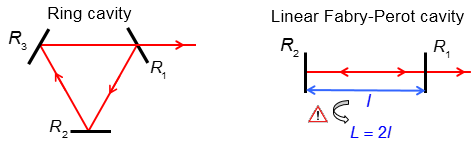
\includegraphics[scale=0.6]{ch3/image2.png}
	\captionof{figure}{ }
	\end{wrapfigure}
Il existe deux type de cavité : la cavité circulaire et la linéaire de type Fabry-Perot. S'il 
n'y a pas de pertes, le champ lors de la $n+1^e$ résonance dans la cavité vaut celui de la $n^e$ 
résonance avec un terme de phase
\begin{equation}
\mathcal{E}_{n+1}=\mathcal{E}_{n}\exp(ikL)
\end{equation}
Ce qui donne lieu à une résonance pour $kL = m2\pi$. 

\newpage
	\begin{wrapfigure}[5]{l}{3cm}
	\vspace{-2mm}
	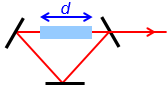
\includegraphics[scale=0.6]{ch3/image3.png}
	\captionof{figure}{ }
	\end{wrapfigure}
Avec $k=\omega/c$, on trouve que les modes 
longitudinaux (équidistants en fréquence, mais \textbf{pas} en longueur d'onde) de la cavité sont caractérisé par 
\begin{equation}
\omega_m = m\dfrac{2\pi}{L}c
\end{equation}
où l'indice de réfraction du milieu a été omis (mais il faut garder à l'esprit qu'il existe). Si 
l'on insère un milieu à gain dans la cavité
\begin{equation}
{\nu _{\rm{m}}} = mc\left(\frac{1}{{{\eta _c}(L - d) + {\eta _L}d}}\right)
\end{equation}

Cependant, pour avoir un laser, il faut forcément des pertes : un des miroirs doit être un 
semi-miroir. Dans le cas idéal, on pourrait imaginer l'utilisation de miroirs 100\% sauf un 
et pas d'autres pertes. Nous faisons l'hypothèses que les variations dues à l'atténuation sont 
petites.
\begin{itemize}
\item[$\bullet$] Réflexivité $R_j<1$
\item[$\bullet$] Pertes internes (diffusion,\dots) : $\alpha_j$
\item[$\bullet$] Sur une résonance, peu de variation : $R_j\approx1, \alpha_i\ll 1$
\end{itemize}\ 


	\begin{wrapfigure}[6]{r}{4cm}
	\vspace{-20mm}
	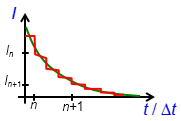
\includegraphics[scale=0.8]{ch3/image4.png}
	\captionof{figure}{ }
	\end{wrapfigure}
Pour une cavité circulaire\footnote{Notons que cette formule est valable même en cas de forte pertes.}
\begin{equation}
{I_{n + 1}} = {R_1}{R_2}{R_3}{e^{ - {\alpha _i}L}}{I_n}
\end{equation}
Si l'on adopte le point de vue d'un modèle continu sur un tour de cavité
\begin{equation}
\frac{{dI}}{{dt}} =  - I/{t_c}
\label{eq:DefDI}
\end{equation}
où $t_c$ est le temps de vie d'un photon dans la cavité (on fait un flash et on compte le temps 
qu'il faut pour que le photon redescende). Après intégration
\begin{equation}
{I_{n + 1}} = {e^{ - \Delta t/{t_c}}}{I_n}
\end{equation}
où $\Delta t= L/c$. Les deux modèles sont très proche, nous pouvons égaler les expressions de 
${I_{n + 1}}$ pour en trier
\begin{equation}
 \Rightarrow 1/{t_c} = {K_c} = {\alpha _i}c - \frac{c}{L}\ln ({R_1}{R_2}{R_3})
\end{equation}
Connaissant $K_c$, on peut écrire une équation différentielle qui décrit l'évolution de 
l'amplitude du champ dans une cavité vide. En partant de \eqref{eq:DefDI} 
\begin{equation}
{\dot {\cal E}} =  - \frac{{{K_c}}}{2}{{\cal E}}
\label{eq:CalE}
\end{equation}
où ${\dot {\cal E}}$ est l'amplitude du champ électrique, $\omega=\omega_m$ et le $1/2$ 
vient du lien entre intensité et amplitude.\\

	\begin{wrapfigure}[6]{l}{5cm}
	\vspace{-5mm}
	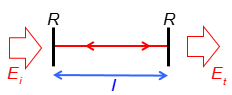
\includegraphics[scale=0.8]{ch3/image5.png}
	\captionof{figure}{ }
	\end{wrapfigure}
La fonction de transfert d'une cavité Fabry-Pérot est donné par
\begin{equation}
{\left| {{E_t}} \right|^2} = \frac{{{{\left| {{E_i}} \right|}^2}}}{{1 + \frac{{4R}}{{{{(1 - R)}^2}}}{{\sin }^2}(kl)}}
\end{equation}
Il s'agit d'une fonction d'Airy qui est fonction de la finesse. Plus la finesse est grande, plus 
il y aura d'aller-retours dans la cavité et plus les pics (en transmission) deviennent étroits. \\

\newpage
Sous les conditions 
\begin{itemize}
\item[$\bullet$] Bonne cavité : $R\approx1\rightarrow \ln(R)\approx 1-R$
\item[$\bullet$] Proche de la résonance : $\omega=\omega_m+\delta\omega \rightarrow {\sin ^2}(kl) = {\sin ^2}(\frac{{{\omega _m} + \delta \omega }}{c}l) \approx {(\frac{{\delta \omega }}{c}l)^2}$
\item[$\bullet$] Pas de pertes internes distribuées : $\alpha_j=0\rightarrow {K_c} =  - (c/l)\ln (R)$
\end{itemize}\ 


	\begin{wrapfigure}[6]{r}{6cm}
	\vspace{-5mm}
	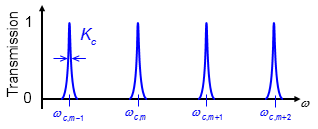
\includegraphics[scale=0.8]{ch3/image6.png}
	\captionof{figure}{ }
	\end{wrapfigure}
La fonction de transfert devient
\begin{equation}
{\left| {{E_t}} \right|^2} \approx \frac{{{{\left| {{E_i}} \right|}^2}}}{{1 + \frac{4}{{\ln {{(R)}^2}}}{{(\frac{{\delta \omega }}{c}l)}^2}}} = \frac{{{{\left| {{E_i}} \right|}^2}}}{{1 + \frac{{\delta {\omega ^2}}}{{{{({K_c}/2)}^2}}}}}
\end{equation}
On en tire le spectre du champ électromagnétique
\begin{equation}
{\left| {\tilde {\cal E}} \right|^2} = \frac{{{{\left| {{{\tilde {\cal E}}_0}} \right|}^2}}}{{1 + \frac{{\delta {\omega ^2}}}{{{{({K_c}/2)}^2}}}}}
\end{equation}
qui est solution de \eqref{eq:CalE} pour les C.I. ${{\cal E}}(t = 0) = {{{\cal E}}_0}$.


\subsubsection{Équation de Maxwell du laser}
Pour avoir un laser, il faut que la cavité ai un milieu à gain ($\mathcal{P}\neq 0$). Si l'on se 
décale par rapport à la résonance, des effets de déphasages vont apparaître. En général, la fréquence 
du laser est légèrement différente de celle de cavité car il y a une variation de l'indice de 
réfraction d'un milieu à l'autre. La fréquence du laser $\omega_L$ n'est a priori pas connue : on 
choisi arbitrairement $\omega_c$ comme référence. \\

Le but est de simplifier l'équation d'onde. Pour ça, on va considérer
\begin{itemize}
\item[$\bullet$] $z$ est la direction de propagation et $x,y$ les directions transverses
\item[$\bullet$] $\vec{E},\vec{P}$ ont la même direction (vrai si milieu isotrope et donc le 
tenseur de susceptibilité est scalaire). On utilisera
\begin{equation}
\vec E = 1/2[{\cal E}(z,t){e^{i({k_c}z - {\omega _c}t)}}\vec e + c.c] = 1/2[Ee + c.c.],\qquad
\vec P = 1/2[{\cal P}(z,t){e^{i({k_c}z - {\omega _c}t)}}\vec e + c.c] = 1/2[Pe + c.c.]
\end{equation}
\item[$\bullet$] Les enveloppes ${\cal E}(z,t){\rm{, }}{\cal P}(z,t)$ varient lentement : elle 
varie sur une échelle de temps beaucoup plus grande que la période du champ EM. 
\item[$\bullet$] La fréquence de résonance vaut $\omega_c=k_cc$.
\end{itemize}
Pour simplifier d'avantage, considérons l'équation scalaire 1D : 
\begin{equation}
E = {\cal E}(z,t){{\mathop{\rm e}\nolimits} ^{i({k_c}z - {\omega _c}t)}},\qquad\qquad
P = {\cal P}(z,t){{\mathop{\rm e}\nolimits} ^{i({k_c}z - {\omega _c}t)}}
\end{equation}
En effectuant les dérivées, on trouve
\begin{equation}
\frac{{{\partial ^2}E}}{{\partial {z^2}}} = [\frac{{{\partial ^2}{\cal E}}}{{\partial {z^2}}} + 2i{k_c}\frac{{\partial {\cal E}}}{{\partial z}} - k_c^2{\cal E}]{{\mathop{\rm e}\nolimits} ^{i({k_c}z - {\omega _c}t)}},\quad \frac{{{\partial ^2}E}}{{\partial {t^2}}} = [\frac{{{\partial ^2}{\cal E}}}{{\partial {t^2}}} - 2i{\omega _c}\frac{{\partial {\cal E}}}{{\partial t}} - \omega _c^2{\cal E}]{{\mathop{\rm e}\nolimits} ^{i({k_c}z - {\omega _c}t)}},\quad 
\end{equation}
\begin{equation}
\frac{{{\partial ^2}P}}{{\partial {t^2}}} = [\frac{{{\partial ^2}{\cal P}}}{{\partial {t^2}}} - 2i{\omega _c}\frac{{\partial {\cal P}}}{{\partial t}} - \omega _c^2{\cal P}]{{\mathop{\rm e}\nolimits} ^{i({k_c}z - {\omega _c}t)}}
\end{equation}
Après substitution
\begin{equation}
\frac{{{\partial ^2}{\cal E}}}{{\partial {z^2}}} + 2i{k_c}\frac{{\partial {\cal E}}}{{\partial z}} - k_c^2{\cal E} - \frac{1}{{{c^2}}}\left( {\frac{{{\partial ^2}{\cal E}}}{{\partial {t^2}}} - 2i{\omega _c}\frac{{\partial {\cal E}}}{{\partial t}} - \omega _c^2{\cal E}} \right) = {\mu _0}\left( {\frac{{{\partial ^2}{\cal P}}}{{\partial {t^2}}} - 2i{\omega _c}\frac{{\partial {\cal P}}}{{\partial t}} - \omega _c^2{\cal P}} \right)
\end{equation}
Comme $\omega_c=k_cc$, $k_c^2{\cal E}$ se simplifie avec ${\omega _c^2{\cal E}}$. L'hypothèse de la 
lente variation de l'enveloppe intervient alors. Comme
\begin{equation}
{t_c},{\rm{ }}\Delta t,{\rm{ }}1/\gamma ,{\rm{ 1/(}}{{\cal G}}{v_g}) \gg 1/{\nu _c}
\end{equation}
Ce qui implique que
\begin{equation}
\begin{array}{ll}
|{\partial _z}{\cal E}| \ll {k_c}|{\cal E}| {\rm{       }},&\qquad|{\partial _{zz}}{\cal E}| \ll k_c^2|{\cal E}|{\rm{ }}\\
|{\partial _t}{\cal E}| \ll {\omega _c}|{\cal E}| {\rm{       }},&\qquad|{\partial _{tt}}{\cal E}| \ll \omega _c^2|{\cal E}|\\
|{\partial _t}{\cal P}| \ll {\omega _c}|{\cal P}|       ,&\qquad|{\partial _{tt}}{\cal P}| \ll \omega _c^2|{\cal P}|
\end{array}
\end{equation}
Les dérivées secondes peuvent ainsi être négligées\footnote{Pq?}. Sachant que $\mu_0=1/
(\varepsilon_0c^2)$, 
l'équation s'écrit
\begin{equation}
2i{k_c}\frac{{\partial {\cal E}}}{{\partial z}} + \frac{{2i{\omega _c}}}{{{c^2}}}\frac{{\partial {\cal E}}}{{\partial t}} =  - {\mu _0}\omega _c^2{\cal P}
\end{equation}
Cette équation décrit une "chose" qui se propage a une certaine vitesse : il est possible de choisir 
un repère particulier pour simplifier. Plaçons-nous dans le repère bougeant à la vitesse $c$ : $
z'=z-ct, t'=t$. L'équation devient
\begin{equation}
2i\frac{{{\omega _c}}}{c}\frac{{\partial {\cal E}}}{{\partial z'}} + \frac{{2i{\omega _c}}}{{{c^2}}}\left(\frac{{\partial {\cal E}}}{{\partial t'}} - c\frac{{\partial {\cal E}}}{{\partial z'}}\right) =  - \frac{{\omega _c^2}}{{{\varepsilon _0}{c^2}}}{\cal P}
\end{equation}
Le premier terme se simplifie avec le second terme de la parenthèse pour donner 
\begin{equation}
\frac{{\partial {\cal E}}}{{\partial t}} = \frac{{i{\omega _c}}}{{2{\varepsilon _0}}}{\cal P}
\end{equation}
On n'observe plus que les variations temporelle de $\mathcal{E}$. C'est normal : le repère se 
déplace à la vitesse $c$ et une lumière qui se propage ne reste pas stationnaire. L'\textbf{équation 
de Maxwell du laser} s'obtient en rajoutant un terme d'amortissement
\begin{equation}
\frac{{\partial {\cal E}}}{{\partial t}} =  - \frac{{{K_c}}}{2}{\cal E} + \frac{{i{\omega _c}}}{{2{\varepsilon _0}}}{\cal P}
\end{equation}
où le second terme obtenu ci-dessus est la réponse du milieu à gain\footnote{Remarque : $K_c$ est l'inverse du temps de vie, il s'agit donc de perte.}. Le slide 9 donne une application de cette 
équation.

\subsection{Équation de Bloch du milieu}
\subsubsection{Polarisation et inversion de la population}
Comme pour chaque modèle, il est nécessaire d'énoncer les différentes hypothèses faites
\begin{itemize}
\item[$\bullet$] Approche semi-classique : le champ EM est classique à fréquence (inconnue) $\omega_L$
\item[$\bullet$] Le milieu a gain contient $N$ atomes par unité de volumes, indépendants et identiques (un seul groupe d'atome, à de l'influence sur ce que ce modèle ne permet pas de décrire (laser à gaz?))
\item[$\bullet$] Seuls les deux niveaux $E_1$ et $E_2$ interagissent avec le champ EM
\item[$\bullet$] Un atome est constitué d'un noyau lourd et d'un électron de charge $-e$
\end{itemize}
\begin{center}
	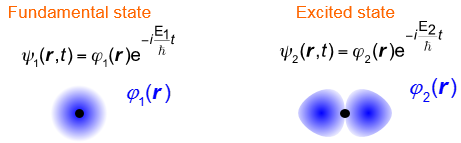
\includegraphics[scale=0.65]{ch3/image7.png}
	\captionof{figure}{ }
\end{center}
Si l'on regarde les états propres de ces atomes, on se rend compte que la densité de probabilité
est stationnaire. Or il faut que les choses bouges sans quoi il n'y aurait pas de radiation.
\begin{equation}
|{\psi _i}({\bf{r}},t){|^2} = |{\varphi _i}({\bf{r}}){|^2}
\end{equation}
Pour palier à ce problème, on introduit une superposition cohérente
\begin{equation}
\psi ({\bf{r}},t) = {c_1}{\psi _1}({\bf{r}},t) + {c_2}{\psi _2}({\bf{r}},t)
\end{equation}
où $|{c_1}{|^2} + |{c_2}{|^2} = 1$ et $|c_i|^2$ est la probabilité que cet atome se trouve dans 
l'état $i$. Soit $\varepsilon^2$, la probabilité que cet atome soit dans l'état fondamental avec 
$c_2\approx1, c_1=\varepsilon\ll 1$. En remplaçant et en prenant le module carré
\begin{equation}
|\psi {|^2} = |{\varphi _2}({\bf{r}}){|^2} + {\varepsilon ^2}|{\varphi _1}({\bf{r}}){|^2} + 2{\rm{Re[}}\varepsilon \varphi _1^*{\varphi _2}{e^{ - i({{\rm{E}}_2} - {{\rm{E}}_1})t/\hbar }}]
\end{equation}
Ici, la densité de probabilité oscille à la fréquence $\omega_a = (E_2-E_1)/\hbar$, il va donc 
y avoir radiation d'énergie par émission de photon à l'énergie $\hbar\omega_a$.\\

	\begin{wrapfigure}[8]{r}{5cm}
	\vspace{-5mm}
	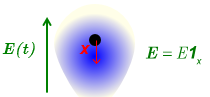
\includegraphics[scale=0.86]{ch3/image9.png}
	\captionof{figure}{ }
	\end{wrapfigure}
Regardons maintenant ce qui se passe au niveau de la polarisation macroscopique
\begin{equation}
\vec{P}: N\vec{p_a}
\end{equation}
où ${{\bf{p}}_a} =  - e\left\langle {\bf{r}} \right\rangle  =  - e\left\langle \psi  \right|{\bf{x}}\left| \psi  \right\rangle$
On suppose ici que tous les atomes ont la même polarisation microscopique. Supposons que le 
centre du nuage se déplace selon $x$ et que l'on soit dans l'état de polarisation cohérente où l'on 
suppose que les coefficients peuvent évoluer au cours du temps
\begin{equation}
\left| {\psi (t)} \right\rangle  = {c_1}(t)\left| {{\psi _1}} \right\rangle  + {c_2}(t)\left| {{\psi _2}} \right\rangle 
\end{equation}
où $\left| {{\psi _j}} \right\rangle  = \left| {{\varphi _j}} \right\rangle {\rm{exp(}} - i\frac{{{{\rm{E}}_j}}}{\hbar }t{\rm{)}}$, ${{H}_0}\left| {{\varphi _j}} \right\rangle  = {{\rm{E}}_j}\left| {{\varphi _j}} \right\rangle$ avec $H_0$ l'Hamiltonien de l'atome non perturbé. Sachant que 
la densité d'atome dans l'état propre d'énergie $E_j$ vaut $N|c_j|^2$, on trouve
\begin{equation}
{p_a} =  - e\left\langle {c_1^*{\psi _1} + c_2^*{\psi _2}} \right|x\left| {{c_1}{\psi _1} + {c_2}{\psi _2}} \right\rangle  =  - e\left[ {c_1^*{c_2}\left\langle {{\varphi _1}} \right|x\left| {{\varphi _2}} \right\rangle {{\rm{e}}^{ - i{\omega _a}t}} + c_2^*{c_1}\left\langle {{\varphi _2}} \right|x\left| {{\varphi _1}} \right\rangle {{\rm{e}}^{ + i{\omega _a}t}}} \right]
\end{equation}
En effet, pas mal de termes sont nuls car $\left\langle {{\psi _j}} \right|x\left| {{\psi _j}} \right\rangle  = 0$ (le moment dipolaire d'un atome dans ses états propres est nul).\\

Posons ${\mu _{21}} =  - e\left\langle {{\varphi _1}} \right|x\left| {{\varphi _2}} \right\rangle $ le \textit{moment dipolaire de la transition $2\to1$}. On peut alors écrire
\begin{equation}
 \Rightarrow {p_a} = c_1^*{c_2}{\mu _{21}}{{\rm{e}}^{ - i{\omega _a}t}} + c_2^*{c_1}\mu _{21}^*{{\rm{e}}^{ + i{\omega _a}t}}
\end{equation}
où ${\mu _{12}} = \mu _{21}^*$. Selon la définition $P = N{p_a} = 1/2[{\cal P}{{\rm{e}}^{ - i{\omega _c}t}} + c.c]$ et pas identification avec celle-ci (le premier terme ensemble et le c.c. ensemble) :
\begin{equation}
{\cal P}(t) = 2Nc_1^*{c_2}{\mu _{21}}{\rm{exp[}} - i({\omega _a} - {\omega _c})t]
\label{eq:ch3.1}
\end{equation}
où $\mathcal{P}$ est l'enveloppe de variation lente. Le souci est que jusqu'ici, la variation 
temporelle des coefficients est inconnues. Pour se faire, nous allons résoudre l'équation de 
Schrödinger pour un système perturbé par un champ électrique $\vec{E}$
\begin{equation}
i\hbar \frac{{\rm{d}}}{{{\rm{dt}}}}\left| {\psi (t)} \right\rangle  = {H}\left| {\psi (t)} \right\rangle 
\end{equation}
où $H=H_0+H_{int}$ avec $H_0$ l'Hamiltonien de l'atome non perturbé : $\DS\left\{\begin{array}{ll}
{{H}_0}\left| {{\varphi _1}} \right\rangle  &= {{\rm{E}}_1}\left| {{\varphi _1}} \right\rangle  = \hbar {\omega _1}\left| {{\varphi _1}} \right\rangle\\
{{H}_0}\left| {{\varphi _2}} \right\rangle  &= {{\rm{E}}_2}\left| {{\varphi _2}} \right\rangle  = \hbar {\omega _2}\left| {{\varphi _2}} \right\rangle
\end{array}\right.$. \\

Nous sommes ici dans un chapitre traitant de la théorie semi classique : on fait l'approximation 
que le champ EM est uniforme à l'échelle de la taille de l'atome pour pouvoir écrire que 
$H_{int} = exE$ où $W=-\vec{P}.E$ l'énergie d'un dipôle dans un champ $\vec{E}$ uniforme où 
$\vec{E}$ est polarisé linéairement selon l'axe $x$.\\

En substituant le tout dans Schrödinger 
$\left| {\psi (t)} \right\rangle  = {c_1}\left| {{\varphi _1}} \right\rangle {\rm{exp( - }}i{\omega _1}t{\rm{)}} + {c_2}\left| {{\varphi _2}} \right\rangle {\rm{exp( - }}i{\omega _2}t{\rm{)}}$ on 
trouve
\begin{equation}
i\hbar [({{\dot c}_1} - i{\omega _1}{c_1})\left| {{\varphi _1}} \right\rangle {{\rm{e}}^{ - i{\omega _1}t}} + ({{\dot c}_2} - i{\omega _2}{c_2})\left| {{\varphi _2}} \right\rangle {{\rm{e}}^{ - i{\omega _2}t}}]  = [{\mathbf{H}_0} + exE]({c_1}\left| {{\varphi _1}} \right\rangle {{\rm{e}}^{ - i{\omega _1}t}} + {c_2}\left| {{\varphi _2}} \right\rangle {{\rm{e}}^{ - i{\omega _2}t}})
\end{equation}
Par projection sur $\bra{\varphi_1}$
\begin{equation}
(i\hbar {\dot c_1} + \underbrace{\hbar {\omega _1}}_{E_1}{c_1}){{\rm{e}}^{ - i{\omega _1}t}} = ({{\rm{E}}_1} + eE\underbrace{\left\langle {{\varphi _1}} \right|x\left| {{\varphi _1}} \right\rangle }_{=0} ){c_1}{{\rm{e}}^{ - i{\omega _1}t}} + eE\left\langle {{\varphi _1}} \right|x\left| {{\varphi _2}} \right\rangle {c_2}{{\rm{e}}^{ - i{\omega _2}t}}
\end{equation}
car il n'y a pas de moment dipolaire permanent (les éléments de matrices diagonaux sont nuls, ceci 
car la fonction est de parité paire ou impaire). On trouve alors une équation pour $c_1$
\begin{equation}
{\dot c_1} = \frac{{ - i}}{\hbar }eE\left\langle {{\varphi _1}} \right|x\left| {{\varphi _2}} \right\rangle {c_2}{{\rm{e}}^{ - i{\omega _a}t}}
\end{equation}
En projetant sur $\bra{\varphi_2}$, on trouve
\begin{equation}
{\dot c_2} = \frac{{ - i}}{\hbar }eE\left\langle {{\varphi _2}} \right|x\left| {{\varphi _1}} \right\rangle {c_1}{{\rm{e}}^{ + i{\omega _a}t}}
\end{equation}
Nos deux coefficients sont alors donnés par
\begin{equation}
{\dot c_1} = \frac{i}{\hbar }{\mu _{21}}{c_2}E{{\rm{e}}^{ - i{\omega _a}t}},\qquad\qquad
{\dot c_2} = \frac{i}{\hbar }\mu _{21}^*{c_1}E{{\rm{e}}^{ + i{\omega _a}t}}
\label{eq:ch3.2}
\end{equation}
Il serait intéressant de trouver une équation liant \eqref{eq:ch3.1} et \eqref{eq:ch3.2}. Pour 
se faire, il suffit de différencier \eqref{eq:ch3.1}
\begin{equation}
\dot {\cal P}(t) =  - i({\omega _a} - {\omega _c}){\cal P}(t) + 2N{c_2}{\mu _{21}}{{\rm{e}}^{ - i({\omega _a} - {\omega _c})t}}\underbrace{(\frac{{ - i}}{\hbar })\mu _{21}^*c_2^*E{{\rm{e}}^{ + i{\omega _a}t}}}_{\dot{c_1}^*} + 2Nc_1^*{\mu _{21}}{{\rm{e}}^{ - i({\omega _a} - {\omega _c})t}}\underbrace{(\frac{i}{\hbar })\mu _{21}^*{c_1}E{{\rm{e}}^{ + i{\omega _a}t}}}_{\dot{c_2}}
\end{equation}
On voit apparaître les coefficients et leur conjugué, il est possible de faire apparaître les 
modules carrés
\begin{equation}
\dot {\cal P}(t) =  - i({\omega _a} - {\omega _c}){\cal P}(t) + 2N\frac{i}{\hbar }|{\mu _{21}}{|^2}(|{c_1}{|^2} - |{c_2}{|^2}){\rm{exp(}}i{\omega _c}t{\rm{)}}E
\end{equation}
où $E = \frac{1}{2}[{\cal E}(t){{\rm{e}}^{ - i{\omega _c}t}} + {{\cal E}^*}(t){{\rm{e}}^{i{\omega _c}t}}]$. On peut négliger le terme en $\mathcal{E}^*$ car il va générer des oscillations à $2\omega_c$ 
ce qui est trop rapide que pour être perçu dans la moyenne.\\

On définit alors l'\textbf{inversion de population} $\mathcal{D}(t) : N(|c_2|^2-|c_1|^2) = N_2-N_1$ 
\begin{equation}
\dot {\cal P}(t) =  - i({\omega _a} - {\omega _c}){\cal P}(t) - \frac{i}{\hbar }|{\mu _{21}}{|^2}{\cal D}{\cal E}
\end{equation}
Le problème est que nous ne savons pas comment cette inversion de population varie. Pour se faire, 
dérivons $\mathcal{D}$
\begin{equation}
\dot {\cal D}(t) = N({\dot c_2}c_2^* + {c_2}\dot c_2^* - {\dot c_1}c_1^* - {c_1}\dot c_1^*)
\end{equation}
Sachant que
\begin{equation}
\left\{\begin{array}{ll}
N{\dot c_1}c_1^* = Nc_1^*\frac{i}{\hbar }{\mu _{21}}{c_2}E{{\rm{e}}^{ - i{\omega _a}t}} = \frac{i}{\hbar }\frac{1}{2}{\cal P}{{\rm{e}}^{ - i{\omega _c}t}}E =  - N\dot c_2^*{c_2}\\
N{\dot c_2}c_2^* = Nc_2^*\frac{i}{\hbar }\mu _{21}^*{c_1}E{{\rm{e}}^{ + i{\omega _a}t}} = \frac{i}{\hbar }\frac{1}{2}{{\cal P}^*}{{\rm{e}}^{ + i{\omega _c}t}}E =  - N\dot c_1^*{c_1}
\end{array}\right.
\end{equation}
On peut ré-écrire $\dot{\mathcal{D}}$
\begin{equation}
\dot {\cal D}(t) =  - \frac{i}{\hbar }({\cal P}{{\rm{e}}^{ - i{\omega _c}t}} - {{\cal P}^*}{{\rm{e}}^{ + i{\omega _c}t}})E
\end{equation}
Sachant que $E = \frac{1}{2}[{\cal E}(t){{\rm{e}}^{ - i{\omega _c}t}} + {{\cal E}^*}(t){{\rm{e}}^{i{\omega _c}t}}]$
\begin{equation}
\dot {\cal D}(t) =  - \frac{i}{{2\hbar }}({\cal P}{{\cal E}^*} - {\cal E}{{\cal P}^*}) - \frac{i}{{2\hbar }}({\cal P}{\cal E}{{\rm{e}}^{ - 2i{\omega _c}t}} - {{\cal P}^*}{{\cal E}^*}{{\rm{e}}^{ + 2i{\omega _c}t}})
\end{equation}
où le dernier terme est nul, la fréquence d'oscillation étant trop élevée. Nous avons alors établi
l'équation régissant l'évolution de l'inversion de population
\begin{equation}
\dot {\cal D}(t) =  - \frac{i}{{2\hbar }}({\cal P}{{\cal E}^*} - {\cal E}{{\cal P}^*})
\end{equation}



\subsubsection{Termes de relaxation et de pompe}
\textsc{A. Amortissement de la polarisation macroscopique}\\
Le système d'équation \eqref{eq:ch3.2} montre que $c_i\propto E$ : si le champ est nul et que 
l'atome est excité alors l'atome reste indéfiniment dans cet état. Ceci n'est pas possible et 
cette aberration vient du fait que \eqref{eq:ch3.2} ne tien compte que des interactions 
cohérentes mais il faut également tenir compte que les niveaux d'énergies ont un temps de vie fini, 
ces amplitudes de probabilité doivent donc décroie même en absence de champ.\\

Supposons $E=0$. Soit $|c_j|^2$ la probabilité que le système soit dans l'état $j$ et 
$1/\gamma_j$ le temps de vie dans l'état $j$
\begin{equation}
\begin{array}{l}
|{c_1}{|^2} \propto {\rm{exp(}} - {\gamma _1}t{\rm{)}}\\
|{c_2}{|^2} \propto {\rm{exp(}} - {\gamma _2}t{\rm{)}}
\end{array}\qquad\Rightarrow\qquad\begin{array}{l}
{c_1} \propto {\rm{exp(}} - {\gamma _1}t/2{\rm{)}}\\
{c_2} \propto {\rm{exp(}} - {\gamma _2}t/2{\rm{)}}
\end{array}
\end{equation}
Avec \eqref{eq:ch3.1} : ${\cal P}(t) \propto c_1^*{c_2}$ et comme
${\cal P}(t) \propto \exp ( - \frac{{{\gamma _1} + {\gamma _2}}}{2}t)$, on en tire
\begin{equation}
\dot {\cal P}(t) =  - {\gamma _ \bot }{\cal P},\qquad \text{où }\ {\gamma _ \bot } = ({\gamma _1} + {\gamma _2})/2
\end{equation}
Ce terme $\gamma_\perp$ est un terme d'amortissement qui permet de tenir compte des dés-excitations 
spontanées.\\

Lorsqu'on parle de la largeur de raie correspondant au profil du gain, il n'y avait pas que le temps 
de vie qui entrait en jeu : il fallait tenir compte des déphasages introduits par les collision. 
Après un certain temps, les dipôles microscopiques deviennent indépendants
\begin{equation}
\vec{P} \neq N\vec{p_a}
\end{equation}
Il faut donc modifier l'expression\footnote{Le $2$ avec 
$\tau_0$ vient du fait qu'il y a deux polarisations} du $\gamma_\perp$
\begin{equation}
{\gamma _ \bot } = \frac{1}{2}\left({\gamma _1} + {\gamma _2} + \frac{1}{{{t_{nr1}}}} + \frac{1}{{{t_{nr2}}}} + \frac{2}{{{\tau _0}}}\right)
\end{equation}
On trouve alors la \textbf{première équation de Bloch}\\

\retenir{
\begin{equation}
\dot {\cal P}(t) =  - {\gamma _ \bot }{\cal P} - i({\omega _a} - {\omega _c}){\cal P}(t) - \frac{i}{\hbar }|{\mu _{21}}{|^2}{\cal D}{\cal E}
\end{equation}
où le premier terme est l'amortissement de $\mathcal{P}$, le second met en évidence la différence de 
fréquence entre la cavité et le laser qui veulent tous deux avoir leur résonance et le 
troisième terme le couplage entre le champ EM et le milieu atomique.}\ \\

\textsc{Amortissement de $\mathcal{D}$ et terme de pompe}\\
Nous avons pour l'instant procéder de façon très générale en tenant compte de l'amortissement de 
la densité de population. On se rend bien compte qu'il faut un mécanisme qui mette le système 
hors équilibre pour que $N_1\ll N_2$ de façon à avoir émission laser. On va donc procéder à un 
pompage incohérent dont le but est de créer une inversion de la population\footnote{Celui-ci est 
indépendant du fait que le milieu lasse.} (collisions, pompage optique, électrique,\dots)\footnote{D'où vient ce truc ?}
\begin{equation}
{\dot {\cal D}} =  + {\gamma _\parallel }{\hat {\cal D}} +  \cdots 
\end{equation}
où $\hat{\mathcal{D}}$ est le \textbf{coefficient de pompe}. On en tire la \textbf{deuxième équation 
de Bloch}\\

\retenir{\begin{equation}
\dot {\cal D}(t) =  - \frac{i}{{2\hbar }}({\cal P}{{\cal E}^*} - {\cal E}{{\cal P}^*}) - {\gamma _\parallel }({{\cal D}} - {\hat {\cal D}})
\end{equation}
où le premier terme est le couplage entre le champ EM et le milieu et le second le terme d'amortissement et de pompage.}\ \\

\theor{\textsc{Equation de Maxwell-Bloch pour le laser}

\begin{equation}
\begin{array}{ll}
\dot {\cal E}(t) &\DS=  - \frac{{{K_c}}}{2}{\cal E} + \frac{{i{\omega _c}}}{{2{\varepsilon _0}}}{\cal P}\\
\dot {\cal P}(t) &\DS=  - {\gamma _ \bot }{\cal P} - \frac{i}{\hbar }|{\mu _{21}}{|^2}{\cal D}{\cal E} - i({\omega _a} - {\omega _c}){\cal P}(t)\\
\dot {\cal D}(t) &\DS=  - {\gamma _\parallel }({{\cal D}} - {\hat {\cal D}}) - \frac{i}{{2\hbar }}({\cal P}{{\cal E}^*} - {\cal E}{{\cal P}^*})
\end{array}
\end{equation}
où $\mathcal{E},\mathcal{P}$ sont des enveloppes complexe variant lentement et $\mathcal{D}$ est 
réel.
}\ \\

\section{État stationnaire d'un laser}
Le slide 20 détaille une longue étape mathématique ayant pour but d'écrire la relation d'inversion
de population. Les équations importantes sont
\begin{equation}
[{K_c}/2 - i({\omega _L} - {\omega _c})]{{\cal E}_0} = \frac{{i{\omega _c}}}{{2{\varepsilon _0}}}{{\cal P}_0}
\label{eq:3prim}
\end{equation}
\begin{equation}
{{\cal P}_0} = \frac{{|{\mu _{21}}{|^2}}}{\hbar }\frac{{{\cal D}{{\cal E}_0}}}{{({\omega _L} - {\omega _a}) + i{\gamma _ \bot }}}
\label{eq:4prim}
\end{equation}
Avec celles-ci, on en tire
\begin{equation}
{{\cal D}} = {{{\hat {\cal D}}} \mathord{\left/
 {\vphantom {{{\hat {\cal D}}} {\left[ {1 + \frac{{|{{\cal E}_0}{|^2}}}{{{{{\cal I}}_s}}}\frac{1}{{1 + {{[({\omega _L} - {\omega _a})/{\gamma _ \bot }]}^2}}}} \right]}}} \right.
 \kern-\nulldelimiterspace} {\left[ {1 + \frac{{|{{\cal E}_0}{|^2}}}{{{{{\cal I}}_s}}}\frac{1}{{1 + {{[({\omega _L} - {\omega _a})/{\gamma _ \bot }]}^2}}}} \right]}}
\label{eq:5prim}
\end{equation}
Lorsque $\omega_L=\omega_a$ la cavité est accordée :
\begin{equation}
{{\cal D}} = \frac{{{\hat {\cal D}}}}{{1 + |{{\cal E}_0}{|^2}/{{{\cal I}}_s}}}
\end{equation}
On parle de \textbf{saturation de l'inversion de population} où $\mathcal{I}_s$ est l'intensité de 
saturation qui ne dépend que des paramètres du milieu. On peut remarquer que plus l'intensité est 
élevée, plus l'inversion de population est petite. On remarque en effet que l'inversion est plus 
faible en présence d'un champ EM car celui-ci provoque de l'émission stimulée qui tend à diminuer
cette inversion de population. 

\subsection{Intensité laser et inversion de population}
Considérons $\omega_c=\omega_a=\omega_L$. Si on n'a pas de champ $\mathcal{E}_0=0$, pas de dipôle, polarisation nulle $\mathcal{P}_0=0$ et $\mathcal{D}=\hat{\mathcal{D}}$. Ceci est la solution 
triviale mais il en existe une autre. Sachant que 
\begin{equation}
{K_c}{{\cal E}_0} = \frac{{i{\omega _c}}}{{{\varepsilon _0}}}{{\cal P}_0},\qquad\qquad 
{{\cal P}_0} =  - i\frac{{|{\mu _{21}}{|^2}}}{{\hbar {\gamma _ \bot }}}{\cal D}{{\cal E}_0}
\end{equation}
On en tire
\begin{equation}
 - i\frac{{|{\mu _{21}}{|^2}}}{{\hbar {\gamma _ \bot }}}{\cal D}{{\cal E}_0} =  - i\frac{{{K_c}{\varepsilon _0}}}{{{\omega _c}}}{{\cal E}_0}
\end{equation}
Soit encore
\begin{equation}
{\cal D} = {{\cal D}_s} = \frac{{{K_c}{\varepsilon _0}\hbar {\gamma _ \bot }}}{{{\omega _c}|{\mu _{21}}{|^2}}}
\end{equation}
L'inversion de population est "bloquée" à une constante $\mathcal{D}_s$. En terme d'intensité (avec
\eqref{eq:5prim})
\begin{equation}
{{{\cal D}}_s} = \frac{{{\hat {\cal D}}}}{{1\; + |{{\cal E}_0}{|^2}/{{{\cal I}}_s}}}
\qquad\Rightarrow\qquad |{{\cal E}_0}{|^2} = (\frac{{{\hat {\cal D}}}}{{{{{\cal D}}_s}}} - 1){{{\cal I}}_s}
\end{equation}
\begin{center}
	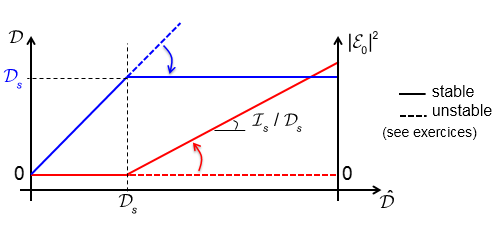
\includegraphics[scale=0.7]{ch3/image8.png}
	\captionof{figure}{Courbes caractéristiques d'un laser}
\end{center}
La première solution $\mathcal{D}<\mathcal{D}_s$ correspond au laser éteint, champ d'intensité nul 
dont la densité de population est directement proportionnelle (il n'y a que de la fluorescence ici). A partir d'un certain moment il y a bifurcation vers une seconde solution et on retrouve la solution 
non triviale pour laquelle l'inversion est bloquée à une constante et l'inversion augmente 
linéairement avec $\hat{\mathcal{D}}$. On nomme alors $\mathcal{D}_s$ le \textit{seuil laser}.\\


\subsection{Susceptibilité électrique et gain}
Reprenons notre équation de polarisation \eqref{eq:4prim} et isolons $\chi(\omega)$
\begin{equation}
{{\cal P}_0} = \frac{{|{\mu _{21}}{|^2}}}{\hbar }\frac{{{\cal D}{{\cal E}_0}}}{{({\omega _L} - {\omega _a}) + i{\gamma _ \bot }}} \equiv {\varepsilon _0}\chi (\omega ){{\cal E}_0}\qquad\Leftrightarrow\qquad
\chi (\omega ) = \frac{{|{\mu _{21}}{|^2}}}{{\hbar {\varepsilon _0}}}\frac{{\cal D}}{{({\omega _L} - {\omega _a}) + i{\gamma _ \bot }}}
\end{equation}
Avec \eqref{eq:5prim}
\begin{equation}
\chi  = \frac{{|{\mu _{21}}{|^2}}}{{\hbar {\varepsilon _0}}}\frac{{{\hat {\cal D}}}}{{{\gamma ^2}_ \bot }}\left( {\frac{{({\omega _L} - {\omega _a}) - i{\gamma _ \bot }}}{{{{({\omega _L} - {\omega _a})}^2} + {\gamma ^2}_ \bot }}} \right)\left( {\frac{{{\gamma ^2}_ \bot  + {{({\omega _L} - {\omega _a})}^2}}}{{1 + |{{\cal E}_0}{|^2}/{{\cal I}_s} + {{[({\omega _L} - {\omega _a})/{\gamma _ \bot }]}^2}}}} \right)
\end{equation}
Après simplification
\begin{equation}
\chi (\omega ) = \frac{{|{\mu _{21}}{|^2}}}{{\hbar {\varepsilon _0}{\gamma _ \bot }}}\hat {\cal D}\frac{{({\omega _L} - {\omega _a})/{\gamma _ \bot } - i}}{{1 + |{{\cal E}_0}{|^2}/{{{\cal I}}_s} + {{[({\omega _L} - {\omega _a})/{\gamma _ \bot }]}^2}}} = \chi ' + i\chi 
\label{eq:ch3.6}
\end{equation}



	\begin{wrapfigure}[8]{l}{11cm}
	\vspace{-5mm}
	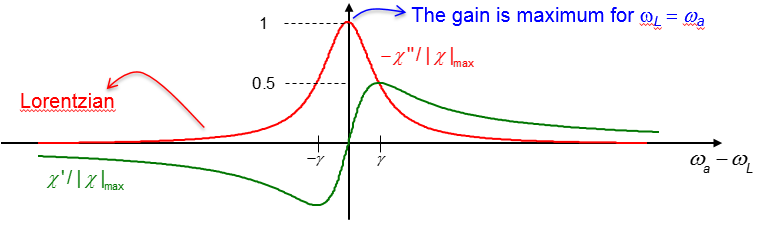
\includegraphics[scale=0.5]{ch3/image10.png}
	\captionof{figure}{ }
	\end{wrapfigure}
	Ce qui semblait compliqué ne l'est pas tellement lorsque l'on trace les courbes. La partie imaginaire(liée au gain ou aux pertes selon le signe) n'est qu'une lorentzienne. Associé à cette résonance, on observe une observation de la partie réelle de la susceptibilité et donc une variation de l'indice de réfraction.\\
	
Le terme $\chi''$ donne le gain ou les pertes. Il apparait un terme $|\mathcal{E}_0|^2/\mathcal{I}_s$ 
qui dépend de l'amplitude du champ
\begin{equation}
\chi  =  - \frac{{|{\mu _{21}}{|^2}}}{{\hbar {\varepsilon _0}{\gamma _ \bot }}}\hat {\cal D}\frac{1}{{1 + |{{\cal E}_0}{|^2}/{{{\cal I}}_s} + {{[({\omega _L} - {\omega _a})/{\gamma _ \bot }]}^2}}}
\end{equation}
où $\DS {{\cal G}} =  - \alpha  =  - \frac{{{\omega _L}}}{c}\chi $. Étudions celle-ci en fonction de l'intensité du champ
\begin{enumerate}
\item \textit{Cas non-sature} ($|\mathcal{E}_0|^2\ll \mathcal{I}_s$.
\begin{equation}
{\cal G} = \frac{{\hbar {\omega _0}B{n_g}}}{c}g({\omega _0})({N_2} - {N_1})
\end{equation}
Il s'agit du cas où l'amplitude du champ est petite par rapport à l'intensité de saturation. Comme le
champ est très petit, nous sommes en dessous du seuil laser et le gain est donné en fonction de la 
fréquence via $g(\omega)$ (une lorentzienne) comme l'expression $\chi''$ ci-dessus. L'avantage est 
que l'on va pouvoir, avec Maxwell-Bloch, tirer par identification un coefficient d'Einstein
\begin{equation}
B \propto |\mu_{21}|^2
\end{equation}
Notons que l'on retrouve la même expression qu'au chapitre 2 pour $g(\omega)$ avec $\gamma_n =
2\gamma_\perp$.
\item \textit{Cas sature} (($\mathcal{I}_s\ll|\mathcal{E}_0|^2 $.)
\begin{equation}
{{\cal G}}(\omega ) = \frac{{{\omega _L}|{\mu _{21}}{|^2}}}{{c\hbar {\varepsilon _0}{\gamma _ \bot }}}\frac{{\hat {\cal D}}}{{1 + |{{\cal E}_0}{|^2}/{{{\cal I}}_s}}}\frac{1}{{1 + {{[(\omega  - {\omega _a})/\gamma ]}^2}}}
\end{equation}
Il n'est plus ici possible de le négliger, mais on peut le mettre en évidence. On retrouve également 
une lorentzienne mais plus large car le "nouveau" $\gamma$ est l'ancien multiplié par un facteur 
supérieur à l'unité
\begin{equation}
{\gamma _ \bot } \to {\rm{ }}\gamma  = {\gamma _ \bot }\sqrt {1 + |{{\cal E}_0}{|^2}/{{{\cal I}}_s}} 
\end{equation}
Il s'agit d'un élargissement homogène de $g(\omega)$ (tous les atomes réagissent de la même façon, 
par exemple avoir un champ dans la cavité rend le spectre plus large car celui-ci crée de l'émission 
stimulée).
\begin{center}
	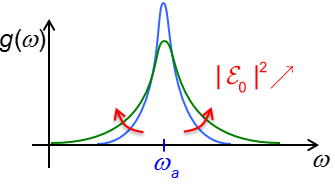
\includegraphics[scale=0.5]{ch3/image11.png}
	\captionof{figure}{$\omega_{c,j}$ est la fréquence angulaire de mode de la cavité. $\omega_{c,0}$
	est la fréquence la plus proche de la fréquence atomique $\omega_a$.}
\end{center}
\end{enumerate}
Une question légitime serait de se demander ce que vaut le gain après la saturation. On sait 
qu'il vaut les pertes ce qui ne saute pas aux yeux en regarder MB. Reprenons \eqref{eq:3prim} et 
\eqref{eq:4prim}
\begin{equation}
{K_c}{{\cal E}_0} = \frac{{i{\omega _c}}}{{{\varepsilon _0}}}{{\cal P}_0},\qquad 
{{\cal P}_0} =  - i\frac{{|{\mu _{21}}{|^2}}}{{\hbar {\gamma _ \bot }}}{\cal D}{{\cal E}_0}
\end{equation}
En combinant les deux, on exprime pour les pertes
\begin{equation}
{K_c} = \frac{{{\omega _L}}}{{{\varepsilon _0}}}\frac{{|{\mu _{21}}{|^2}}}{{\hbar {\gamma _ \bot }}}{{\cal D}_s}
\end{equation}
De l'autre côté, nous avons pour le gain
\begin{equation}
{{\cal G}} =  - \frac{{{\omega _L}}}{c}\chi  = \frac{{{\omega _L}}}{c}\frac{{|{\mu _{21}}{|^2}}}{{\hbar {\varepsilon _0}}}\frac{{\cal D}}{{{\gamma _ \bot }}}
\end{equation}
Comme à la saturation $\mathcal{D}=\mathcal{D}_s$, on arrive à 
\begin{equation}
K_c=c\mathcal{G}
\end{equation}
Ce qui est une solution non triviale pour pertes = gain (condition d'oscillation laser). En 
conclusion en dessous du seuil laser $\hat{\mathcal{D}}_s$, $\mathbb{D}$ et $\mathcal{G}$ garde une 
valeur constante tel que le gain soit égal au pertes. Quand $\hat{\mathcal{D}}$ augmente au 
dessus du seuil, cette augmentation supplémentaire d'énergie est convertie en photons lasant

\subsection{Fréquence du champ laser}
Jusqu'ici nous avions considéré que $\omega_c=\omega_a$ mais que se passe-t-il (pour $\omega_L$) 
si les deux sont différents ? Reprenons \eqref{eq:3prim} et \eqref{eq:4prim}
\begin{equation}
[{K_c}/2 - i({\omega _L} - {\omega _c})]{{\cal E}_0} = \frac{{i{\omega _c}}}{{2{\varepsilon _0}}}{{\cal P}_0},\qquad\qquad
{{\cal P}_0} = \frac{{|{\mu _{21}}{|^2}}}{\hbar }\frac{{{\cal D}{{\cal E}_0}}}{{({\omega _L} - {\omega _a}) + i{\gamma _ \bot }}}
\end{equation}
En substituant l'une dans l'autre
\begin{equation}
[{K_c}/2 - i({\omega _L} - {\omega _c})]{{\cal E}_0} = \frac{{i{\omega _c}}}{{2{\varepsilon _0}}}\frac{{|{\mu _{21}}{|^2}}}{\hbar }\frac{{{\cal D}{{\cal E}_0}}}{{({\omega _L} - {\omega _a}) + i{\gamma _ \bot }}}
\end{equation}
En isolant l'inversion de population
\begin{equation}
\Rightarrow {\cal D} = \frac{{ - 2i{\varepsilon _0}\hbar }}{{{\omega _c}|{\mu _{21}}{|^2}}}[{K_c}/2 - i({\omega _L} - {\omega _c})][({\omega _L} - {\omega _a}) + i{\gamma _ \bot }]
\end{equation}
Il s'agit d'un nombre complexe : comme nous savons que l'inversion de population est réelle, la 
partie imaginaire doit forcément être nulle
\begin{equation}
{\cal D} = \frac{{2{\varepsilon _0}\hbar }}{{{\omega _c}|{\mu _{21}}{|^2}}}\left\{ {\underbrace{- i[\frac{{{K_c}}}{2}({\omega _L} - {\omega _a}) + {\gamma _ \bot }({\omega _L} - {\omega _c})]}_{=0} - ({\omega _L} - {\omega _a})({\omega _L} - {\omega _c}) + \frac{{{K_c}{\gamma _ \bot }}}{2}} \right\}
\label{eq:ch3.7}
\end{equation}
La partie imaginaire étant nulle, on en tire que
\begin{equation}
({\omega _L} - {\omega _a}){K_c}/2 =  - {\gamma _ \bot }({\omega _L} - {\omega _c})
\end{equation}

	\begin{wrapfigure}[12]{l}{10cm}
	\vspace{-5mm}
	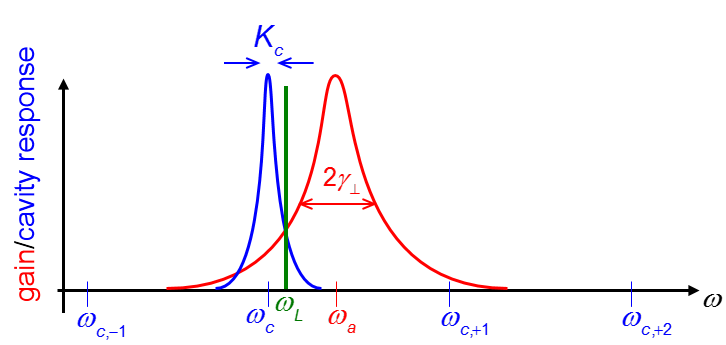
\includegraphics[scale=0.5]{ch3/image12.png}
	\captionof{figure}{ }
	\end{wrapfigure}
Et donc
\begin{equation}
{\omega _L} = \frac{{{\omega _c}2{\gamma _ \bot } + {\omega _a}{K_c}}}{{2{\gamma _ \bot } + {K_c}}}
\end{equation}
La fréquence laser est une sorte de moyenne entre les deux pondérée par le coefficient d'amortissement 
$K_c$ et $2\gamma_\perp=\gamma_h$. Si la cavité est de très haute finesse (par rapport à la largeur 
de la transition atomique), la fréquence laser va coïncider avec celle de la cavité $\omega_c$. 
Inversement, si c'est le milieu atomique qui a une raie très étroite on observera $\omega_L=\omega_a$. 
On nomme $\omega_L$ le terme de \textit{tirage en fréquence}.\\

	\begin{wrapfigure}[12]{r}{10cm}
	\vspace{-5mm}
	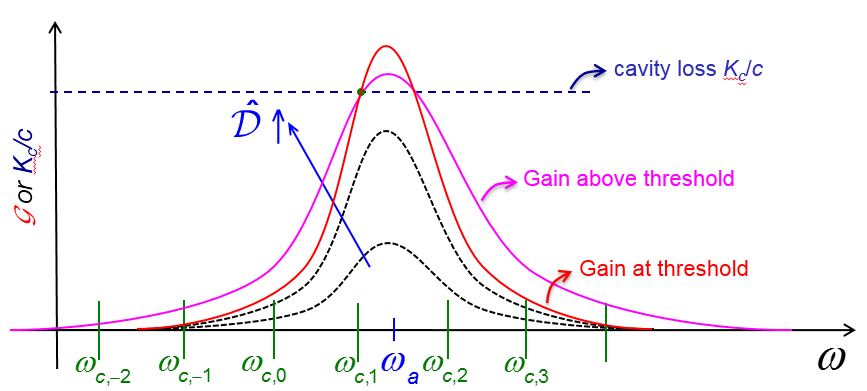
\includegraphics[scale=0.45]{ch3/image13.png}
	\captionof{figure}{ }
	\end{wrapfigure}
Nous avons vu que la forme de raie à tendance à s'élargir lorsque l'on est au delà du seuil laser 
(ceci n'a de sens que si le gain à une largeur qui s'étend sur plusieurs mode). La courbe en noir 
est obtenue lorsque l'on augmente la pompe (de largeur $2\gamma_\perp$). A un moment donné, la 
courbe noire croise la ligne des pertes et donne lieu à la courbe rouge : cela commence à laser. Si 
on augmente encore la puissance le point vert ne va pas changer de place mais nous aurons plus 
d'émission stimulée. Une seule fréquence lasera, les autres, étant en dessous du seuil gain = pertes,
ne laseront pas. \\

Nous venons de voir le cas homogène, regardons ce qu'il en est pour les \textit{lasers with inhomogeneously broadened gain line shape}. En effet, les lasers sont souvent multimodes. Si 
il y a des classes d'atomes, elles auront chacune un mode différent et on peut avoir plusieurs 
émissions laser : régime multimodale. Pour comprendre ceci, regardons l'équation de l'inversion 
de population \eqref{eq:ch3.7}
\begin{equation}
{\cal D} = \frac{{2{\varepsilon _0}\hbar }}{{{\omega _c}|{\mu _{21}}{|^2}}}\left\{ {\frac{{{K_c}{\gamma _ \bot }}}{2} - ({\omega _L} - {\omega _a})({\omega _L} - {\omega _c})} \right\}
\end{equation}
Sachant que $\DS \omega_L-\omega_a =-\frac{{2{\gamma _ \bot }}}{{{K_c}}}({\omega _L} - {\omega _c})$
\begin{equation}
{\cal D} = \frac{{2{\varepsilon _0}\hbar }}{{{\omega _c}|{\mu _{21}}{|^2}}}\frac{{{K_c}{\gamma _ \bot }}}{2}\left\{ {1 + \frac{4}{{{K_c}^2}}{{({\omega _L} - {\omega _c})}^2}} \right\} 
 = {{\cal D}_s}\left\{ {1 + \frac{4}{{{K_c}^2}}{{({\omega _L} - {\omega _c})}^2}} \right\} = {{\cal D}_s}\left\{ {1 + \frac{1}{{{\gamma _ \bot }^2}}{{({\omega _L} - {\omega _a})}^2}} \right\}
\end{equation}
Ici comme $\omega_L\neq\omega_a$, l'inversion de population se fait à $\mathcal{D}>\mathcal{D}_s$ : 
comme il y a un petit décalage entre les résonances, il faut un peu plus d'inversion de population 
que si on était à résonance (nous sommes dans un cas moins optimal, le cas optimal étant $\mathcal{D}\approx\mathcal{D}_s$).\\

	\begin{wrapfigure}[12]{r}{9cm}
	\vspace{-5mm}
	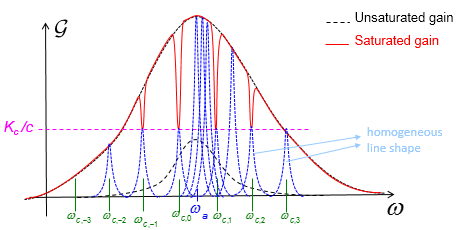
\includegraphics[scale=0.75]{ch3/image14.png}
	\captionof{figure}{ }
	\end{wrapfigure}
La solution stationnaire est représentée en rouge. En noir, il s'agit du cas ou le gain est 
supérieur aux pertes, il va donc y avoir une diminution du gain jusqu'à arriver à la condition où 
le gain vaut les pertes. Il est possible d'avoir un multimode car le fait qu'on ai un lasage à 
un $\omega_c$ n'influence pas le lasage d'un autre $\omega_c$. Entre deux de ces fréquences, 
le champ n'est pas résonant. En l'absence de lasage, le gain peut être supérieur aux pertes. En 
dessous de la ligne en pointillé, il n 'y aura pas de lasage, nous décrivons bien ici un laser 
mutlimode (on parle de trous spectraux, typique He-Ne)\footnote{Paragraphe pas clair, lire slide 31}.\\

	\begin{wrapfigure}[20]{l}{9cm}
	\vspace{-5mm}
	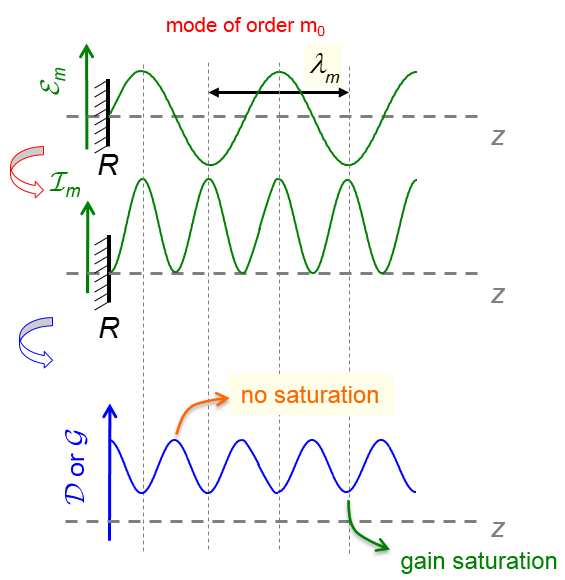
\includegraphics[scale=0.55]{ch3/image15.png}
	\captionof{figure}{ }
	\end{wrapfigure}
La réalité est plus compliquée, car la géométrie joue également un rôle. Nous n'avons pour l'instant
fait aucune différence entre une cavité anneau et FP. Le FP peut donner lieu à des interférences et 
donc une onde stationnaire. En augmentant la pompe pour un mode $\omega_0$ on va rencontrer à un 
certain moment la condition \textit{gain=pertes} donnant lieu à un certain profil d'intensité. Comme 
l'inversion de population varie avec $\mathcal{I}/\mathcal{I}_s$ on crée des trous spatiaux. Si un 
mode se situe juste dans le creux de $\mathcal{G}$ il n'y a pas assez de gain et on n'observera 
jamais de lasage. Par contre, il possible (sur un pic de $\mathcal{G}$) d'avoir un autre lasage car 
la fréquence ne va pas se "nourrir spatialement" au même endroit que le premier mode qui s'est mis à
laser.



































